\documentclass[journal]{IEEEtran}

\usepackage{graphicx}
\usepackage{float}
\usepackage{algorithm}
\usepackage{algorithmic}

\begin{document}
hello world!\cite{edge-ai}

\begin{table}
\centering
\caption{test table}

\begin{tabular}{|c|c|c|}
\hline 
name & class & id \\
\hline
zhangsan & 1 & 0001 \\
\hline
\end{tabular}
\end{table}

\begin{figure}
\centering
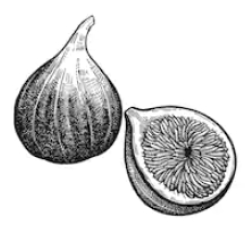
\includegraphics{fig1.png}
\caption{this is a figure}
\end{figure}
\begin{algorithm}
	\caption{A}
	\label{alg:A}
	\begin{algorithmic}
		\STATE {set $r(t)=x(t)$} 
		\REPEAT 
		\STATE set $h(t)=r(t)$ 
		\REPEAT
		\STATE set $h(t)=r(t)$ 
		\UNTIL{B} 
		\UNTIL{B}
	\end{algorithmic}
\end{algorithm}


\bibliographystyle{IEEEtran}
\bibliography{reference}

\end{document}